% ----------------------------------------------------------------------------
% Section 6.4 --- Recovery of the Schwarzschild Metric
% From former §7.4, condensed while preserving all equations
% ----------------------------------------------------------------------------
\subsection{Recovery of the Schwarzschild Metric}
\label{subsec:recovery-of-the-schwarzschild-metric}

For a static, approximately spherically symmetric distribution of
localized projected configurations, the collective reduction of admissible
relaxation ordering admits a simple effective description.

\paragraph{Operational potential from
\texorpdfstring{$\chi$}{χ}-relaxation slowdown.}
The dimensionless lapse-like factor is
\begin{equation}
  N(r) \;\equiv\;
    \frac{D^\chi_{\mathrm{loc}}(r)}{D^\chi_0},
  \qquad 0 < N(r)\le 1 ,
\end{equation}
with the weak-field identification
\begin{equation}
  \frac{D^\chi_{\mathrm{loc}}}{D^\chi_0}
  \;\simeq\; 1 + \frac{\Phi}{c^2},
  \qquad
  \left|\frac{\Phi}{c^2}\right|\ll 1.
  \label{eq:phi_from_slowdown}
\end{equation}

\paragraph{Poisson-like equation and exterior solution.}
In the weak-structure regime:
\begin{equation}
  \nabla^2 \Phi \;\simeq\; 4\pi G_{\mathrm{eff}}\,\rho ,
  \label{eq:poisson_phi}
\end{equation}
yielding, for an isolated spherical source of mass~$M$:
\begin{equation}
  \Phi(r) \;\simeq\; -\frac{G_{\mathrm{eff}} M}{r}.
  \label{eq:phi_point_mass}
\end{equation}

\paragraph{Metric components from
\texorpdfstring{$\Phi$}{Φ}.}
The static spherically symmetric ansatz reads
\begin{equation}
  ds^2 = -N(r)^2 c^2 dt^2 + N(r)^{-2} dr^2
    + r^2 d\Omega^2.
  \label{eq:metric_from_N}
\end{equation}
In the weak-field limit:
\begin{align}
  g_{tt} &\simeq
    -\left(1 + 2\frac{\Phi}{c^2}\right),
  \label{eq:weak_gtt}\\
  g_{rr} &\simeq
    \left(1 + 2\frac{\Phi}{c^2}\right)^{-1}
    \;\simeq\; 1 - 2\frac{\Phi}{c^2},
  \label{eq:weak_grr}
\end{align}
coinciding with the standard Schwarzschild weak-field expansion:
\begin{equation}
  g_{tt} \simeq
    -\left(1-\frac{2G_{\mathrm{eff}}M}{c^2 r}\right),
  \quad
  g_{rr} \simeq
    \left(1-\frac{2G_{\mathrm{eff}}M}{c^2 r}\right)^{-1}.
  \label{eq:schwarzschild_matching}
\end{equation}

\paragraph{Comparison to classic observational tests.}
Gravitational redshift follows directly from $g_{tt}$:
\begin{equation}
  \frac{\nu_{\mathrm{obs}}}{\nu_{\mathrm{emit}}}
  \;\simeq\;
  1 + \frac{\Phi(r_{\mathrm{emit}})
    -\Phi(r_{\mathrm{obs}})}{c^2}.
\end{equation}
Light deflection yields the standard angle
\begin{equation}
  \alpha \;\simeq\;
    \frac{4G_{\mathrm{eff}}M}{b c^2},
\end{equation}
with $b$ the impact parameter.

\begin{figure}[htbp]
  \centering
  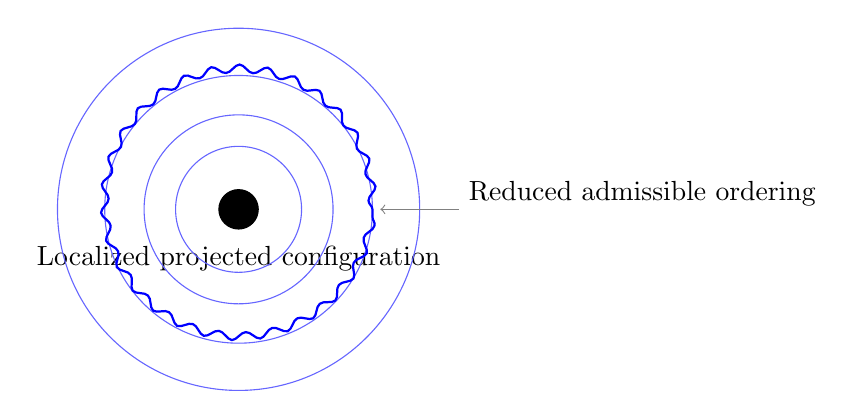
\begin{tikzpicture}[scale=1]
    \filldraw[black] (0,0) circle (0.25);
    \node[below] at (0,-0.35)
      {Localized projected configuration};
    \foreach \r in {0.8,1.2,1.7,2.3} {
      \draw[blue!60] (0,0) circle (\r);
    }
    \draw[blue, thick, decorate,
      decoration={snake, amplitude=0.5mm}]
      (0,0) circle (1.7);
    \draw[->, gray] (2.8,0) -- (1.8,0);
    \node[right] at (2.8,0.2)
      {Reduced admissible ordering};
  \end{tikzpicture}
  \caption{Emergence of Schwarzschild-like behavior.
    A localized projected configuration induces a spatially varying
    reduction of admissible relaxation ordering, manifesting as
    differential proper-time accumulation and emergent metric
    curvature.}
  \label{fig:chi_gravity}
\end{figure}
